\documentclass[a4paper,UTF8]{article}
\usepackage{ctex}
\usepackage[margin=1.25in]{geometry}
\usepackage{color}
\usepackage{graphicx}
\usepackage{amssymb}
\usepackage{amsmath}
\usepackage{amsthm}
\usepackage{enumerate}
\usepackage{bm}
\usepackage{hyperref}
\usepackage{epsfig}
\usepackage{color}
\usepackage{mdframed}
\usepackage{lipsum}
\usepackage{mathtools}
\usepackage{hyperref}
\usepackage{diagbox}
\usepackage{float}
\usepackage{caption}
\usepackage{algorithm}
\usepackage{algorithmicx}  
\usepackage{algpseudocode}
\usepackage{amsmath} 
\usepackage{graphicx}
\usepackage{subfigure}
\newmdtheoremenv{thm-box}{myThm}
\newmdtheoremenv{prop-box}{Proposition}
\newmdtheoremenv{def-box}{定义}
\usepackage{listings}
\usepackage{xcolor}
\lstset{
	numbers=left, 
	numberstyle= \tiny, 
	keywordstyle= \color{ blue!70},
	commentstyle= \color{red!50!green!50!blue!50}, 
	frame=shadowbox, % 阴影效果
	rulesepcolor= \color{ red!20!green!20!blue!20} ,
	escapeinside=``, % 英文分号中可写入中文
	xleftmargin=2em,xrightmargin=2em, aboveskip=1em,
	framexleftmargin=2em
} 

\usepackage{booktabs}

\setlength{\evensidemargin}{.25in}
\setlength{\textwidth}{6in}
\setlength{\topmargin}{-0.5in}
\setlength{\topmargin}{-0.5in}

% \setlength{\textheight}{9.5in}
%%%%%%%%%%%%%%%%%%此处用于设置页眉页脚%%%%%%%%%%%%%%%%%%
\usepackage{fancyhdr}                                
\usepackage{lastpage}                                           
\usepackage{layout}                                             
\footskip = 10pt 
\pagestyle{fancy}                    % 设置页眉                 
\lhead{研一下学期}                    
\chead{论文阅读笔记}                                                
% \rhead{第\thepage/\pageref{LastPage}页} 
\rhead{Step3}                                                                                               
\cfoot{\thepage}                                                
\renewcommand{\headrulewidth}{1pt}  			%页眉线宽,设为0可以去页眉线
\setlength{\skip\footins}{0.5cm}    			%脚注与正文的距离           
\renewcommand{\footrulewidth}{0pt}  			%页脚线宽,设为0可以去页脚线

\makeatletter 									%设置双线页眉                                        
\def\headrule{{\if@fancyplain\let\headrulewidth\plainheadrulewidth\fi%
\hrule\@height 1.0pt \@width\headwidth\vskip1pt	%上面线为1pt粗  
\hrule\@height 0.5pt\@width\headwidth  			%下面0.5pt粗            
\vskip-2\headrulewidth\vskip-1pt}      			%两条线的距离1pt        
 \vspace{6mm}}     								%双线与下面正文之间的垂直间距              
\makeatother  

%%%%%%%%%%%%%%%%%%%%%%%%%%%%%%%%%%%%%%%%%%%%%%
\numberwithin{equation}{section}
%\usepackage[thmmarks, amsmath, thref]{ntheorem}
\newtheorem{theorem}{Theorem}
\newtheorem*{definition}{Definition}
\newtheorem*{solution}{Solution}
\newtheorem*{prove}{Proof}
\newcommand{\indep}{\rotatebox[origin=c]{90}{$\models$}}

\usepackage{multirow}

%--

%--
\begin{document}
\title{论文阅读笔记\\
Step3}
\author{MF1833063, 史鹏, spwannasing@gmail.com}
\maketitle

\newpage
\section{MEMEN: Multi-layer Embedding with Memory Networks for Machine Comprehension}
提出了新的模型:Multi-layer Embedding with Memory Network(MEMEN)。提出了多层embedding,
encoding了word的句法以及语义信息。引入了full-orientation matching。
\begin{figure}[H]
	\centering
	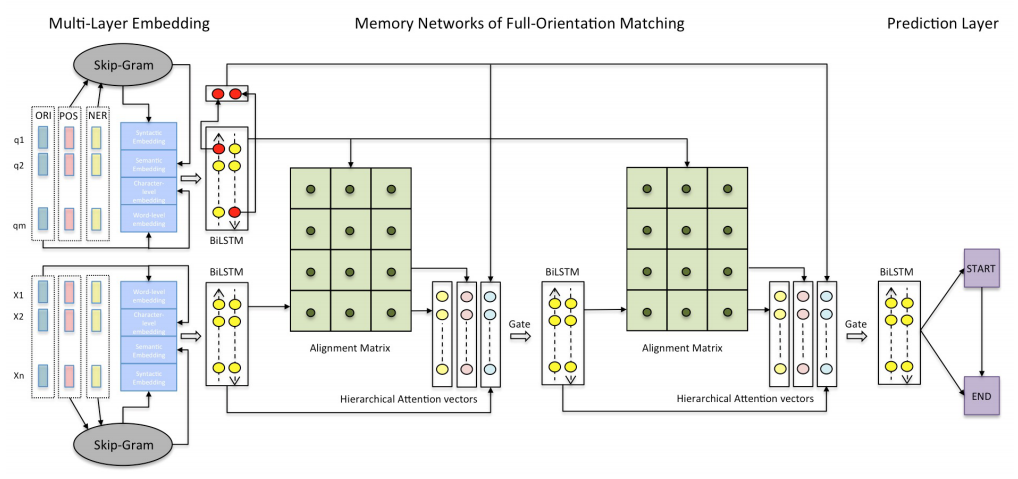
\includegraphics[width=\textwidth]{1-1.png}
	\caption{网络结构图}
\end{figure}
\begin{figure}[H]
	\centering
	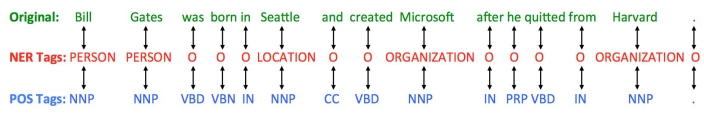
\includegraphics[width=\textwidth]{1-2.png}
	\caption{三种信息的例子}
\end{figure}
\begin{enumerate}
	\item Encoding of Context and Query\\
	$$r_t^P=BiLSTM([w_t^P;c_t^P;s_t^P])$$ 
	$$r_t^Q=BiLSTM([w_t^Q;c_t^Q;s_t^Q])$$
	其中w,c,s分别代表word-level,character-level,tags的embedding,以及query的最后一个隐藏状态$u^Q$
	\item Memory Network of Full-Orientation Matching\\
	\subitem[1] Integral Query Matching\\
	$$c_t = softmax(<u^Q,r_t^P>)$$
	$$m^1=\sum_tc_tr_t^P$$
	\subitem[2] Query-Based Similarity Matching \\
	首先得到alignment matrix $A \in \mathbb{R}^{n\times m}$,$A_{ij}=w_1^T[r_i^P;r_j^Q;r_i^P\circ r_j^Q]$
	$$B = softmax_{row}(A) \in R^{n\times m}$$
	$M^2$的每一列$M^2_t=B \cdot r^Q$
	\subitem[3] Context-Based Similarity Matching \\
	$e=max_{row}(A) \int R^n$,the attention is $d=softmax(e)$
	$$m^3=\sum_tr_t^P\cdot d_t$$

	$$M=f(M^1,M^2,M^3)$$
	$M^1,M^3$是对应的向量重复n次。
	添加额外的gate$$g_t=sigmoid(W_gM)$$ $$M^*=g_t \odot M$$
	$$O_t = BiLSTM(O_{t-1},M)$$
	\item Output Layer\\
	通过Pointer Network来预测答案。首先获取到该网络的初始hidden state:$$z_j=s^Ttanh(W^Qr_j^Q+b^Q)$$
	$$a_i = \frac{exp(z_i)}{\sum exp(z_j)}$$
	$$l_0=\sum a_ir_i^Q$$
	然后Pointer Network:$$z_j^k=c^Ttanh(W^PO_j+W^hl^0$$
	$$a_i^k=\frac{exp(a_i^k)}{\sum exp(z_j^k)}$$
	$$p^k=argmax(a_1^k,...,a_n^k)$$
	k=1,2
	$$v^k=\sum_{i=1}^n a_i^kO_i$$
	$$l_t^1=GRU(l_{t-1},v^k)$$
\end{enumerate}

\newpage
\section{DYNAMIC COATTENTION NETWORKS FOR QUESTION ANSWERING}
因为以前的一些方法都是single-pass,所以没有方法从局部最大恢出来。本篇文章提出了Dynamic Coattention Network (DCN)。
首先是融合问题和文档的相互依赖的表示,以便将重点放在两者的相关部分上。然后Dynamic pointing decoder在潜在的答案范围上迭代。(我理解的这里所谓的迭代法其实就是通过LSTM来decoder)
\begin{figure}[H]
	\centering
	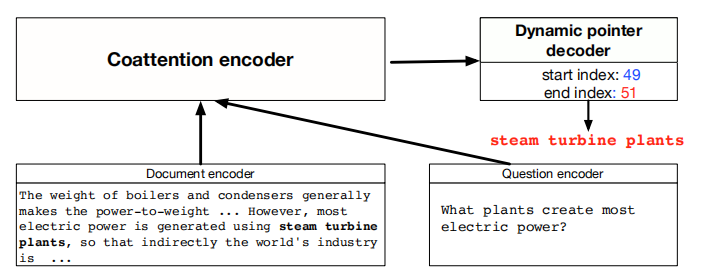
\includegraphics[width=\textwidth]{2-1.png}
	\caption{overview}
\end{figure}
\begin{figure}[H]
	\centering
	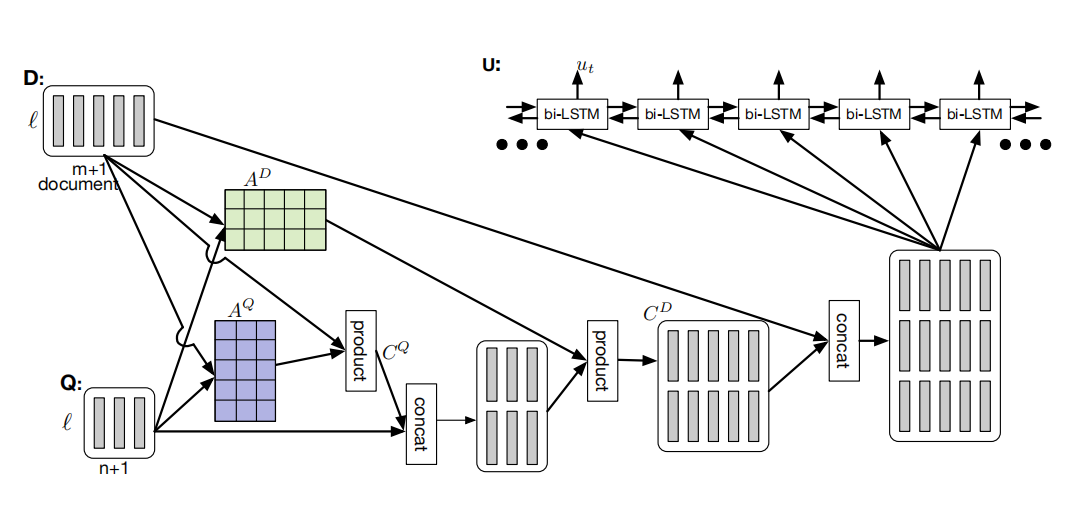
\includegraphics[width=\textwidth]{2-2.png}
	\caption{Coattention encoder.}
\end{figure}

\begin{enumerate}
	\item CoAttention Encoder\\
	首先计算相似度矩阵$L=D^TQ \in \mathbb{R}^{(m+1)\times (n+1)}$,然后得到对应的row-wise与column-wise:
	$$A^Q = softmax (L) \in \mathbb{R}^{(m+1)\times (n+1)}$$
	$$A^D = softmax (L^T) \in \mathbb{R}^{(n+1)\times (m+1)}$$
	$$C^Q=DA^Q \in \mathbb{R}^{l\times (n+1)}$$
	$$C^D=[Q;C^Q]A^D \in \mathbb{R}^{2l\times (m+1)}$$
	这里定义$C^D$就是co-dependent representation of the question and document
	$$u_t = Bi-LSTM(u_{t-1},u_{t+1},[d_d;c_t^D]) \in \mathbb{R}^{2l}$$
	\item Dynamic Pointing Decoder\\
	\begin{figure}[H]
		\centering
		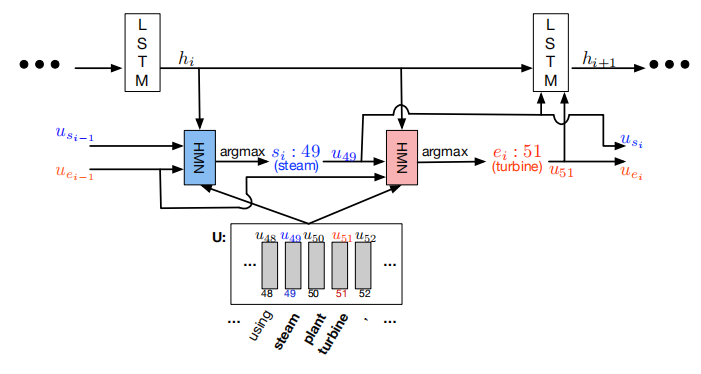
\includegraphics[width=\textwidth]{2-3.png}
		\caption{Dynamic Decode}
	\end{figure}
	在每一个step都会考虑到当前预测的start和end对应的co-attenion的encoding来更新自己的状态。
	$$h_i = LSTM_{dec}(h_{i-1},[u_{s_{i-1}};u_{e_{i-1}}])$$
	$$s_i=\underset{t}{argmax}(\alpha_1,...,\alpha_m)$$
	$$e_i=\underset{t}{argmax}(\beta_1,...,\beta_m)$$
	$\alpha,\beta$的计算类似,下面只介绍$\alpha$
	$$\alpha_t=HMN_{start}(u_t,h_i,u_{s_{i-1}},u_{e_{i-1}})$$
	$$
\begin{aligned} \operatorname{HMN}\left(u_{t}, h_{i}, u_{s_{i-1}}, u_{e_{i-1}}\right) &=\max \left(W^{(3)}\left[m_{t}^{(1)} ; m_{t}^{(2)}\right]+b^{(3)}\right) \\ r &=\tanh \left(W^{(D)}\left[h_{i} ; u_{s_{i-1}} ; u_{e_{i-1}}\right]\right) \\ m_{t}^{(1)} &=\max \left(W^{(1)}\left[u_{t} ; r\right]+b^{(1)}\right) \\ m_{t}^{(2)} &=\max \left(W^{(2)} m_{t}^{(1)}+b^{(2)}\right) \end{aligned}
$$
	\begin{figure}[H]
		\centering
		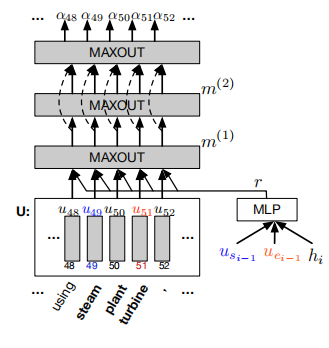
\includegraphics[]{2-5.png}
		\caption{Highway Maxout Network}
	\end{figure}
\end{enumerate}



\newpage
\section{R-NET: MACHINE READING COMPREHENSION WITH SELF-MATCHING NETWORKS}
首先得到question-aware的passage表示,然后提出一种self-matching 注意力机制抽取信息,最后通过pointer Network选择答案。
\begin{figure}[H]
	\centering
	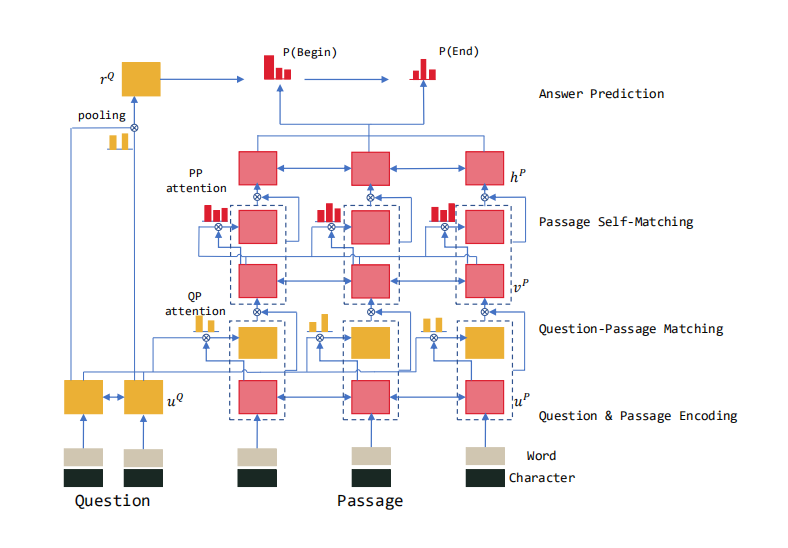
\includegraphics[width=\textwidth]{3-1.png}
\end{figure}
\begin{enumerate}
	\item QUESTION AND PASSAGE ENCODER\\$$u_t^Q=BiGRU_Q(u_{t-1}^Q,[e_t^Q,c_t^Q])$$
	$$u_t^P=BiGRU_P(u_{t-1}^P,[e_t^P,c_t^P])$$
	\item GATED ATTENTION-BASED RECURRENT NETWORKS\\我们提出了一种基于门控注意的递归网络,将问题信息整合到段落表示中.它是一种基于注意力的递归网络的变体,有一个额外的门确定文章中有关问题的信息的重要性。
	$$v_t^P=RNN(v_{t-1}^P,c_t)$$here $c_t=att(u_Q,[u_t^P,v_{t-1}^P])$
	\begin{align*}
		s_j^t&=v^Ttanh(W_u^Qu_j^Q+W_u^Pu_t^P+W_v^Pv_{t-1}^P)\\
		a_i^t&=\frac{exp(s_i^t)}{\sum s_j^t}\\
		c_t&=\sum_{i=1}^m a_i^tu_i^Q 
	\end{align*}
	match-LSTM,将$u_t^P$作为额外的输入。$$v_t^P=RNN(v_{t-1}^P,[u_t^p,c_t])$$
	为了决定passage某部分的重要性以及其相关的question,加了一个额外的gate$$g_t=sigmoid(W_g[u_t^P,c_t])$$
	$$[u_t^P,c_t]^*=g_t \odot [u_t^P,c_t]$$
	\item 剩下的 SELF-MATCHING ATTENTION 以及OUTPUT LAYER都和之前的类似。
\end{enumerate}

\newpage
\section{ReasoNet: Learning to Stop Reading in Machine Comprehension}
引入强化学习,从而能够学得机器应该“阅读”多少次之后,停止迭代。只有正确答案的奖赏是1,其它都是0。
\begin{figure}[H]
	\centering
	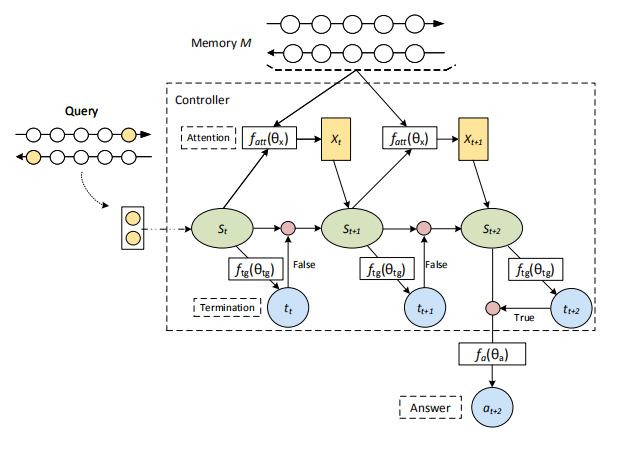
\includegraphics[width=\textwidth]{4-1.png}
\end{figure}

\newpage
\section{FUSIONNET: FUSING VIA FULLY-AWARE ATTENTION WITH APPLICATION TO MACHINE COMPREHENSION}
提出了一个新的概念“history of word”,其实核心思想就是获取到更多的word的表示,将不同level的embedding和词性信息等以及经过神经网络计算后得到的向量都组合在一起,然后在Attention的环节,是计算一组矩阵之间的相似度而不是一组向量。
\begin{figure}[H]
	\centering
	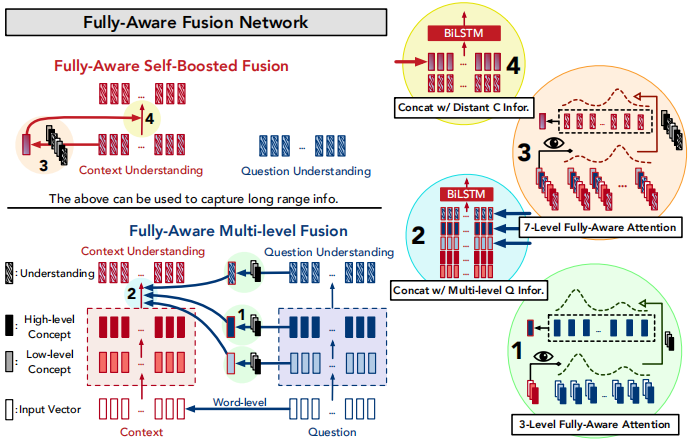
\includegraphics[width=\textwidth]{5-1.png}
\end{figure}
\begin{enumerate}
	\item 首先定义history of the ith word 为$HoW_i$,它是把所有为这个单词生成的表示连接起来。
	\item Fully-Aware Multi-level Fusion
		\subitem[1] Word-level\\
		$$\hat{g}_i^C=\sum_j\alpha_{ij}g_j^Q$$
		where $\alpha_{ij} \propto exp(S(g_i^C,g_j^Q)),S(x,y)=RELU(Wx)^TRELU(Wy)$
		$$\tilde{w}_i^C=[w_i^C,em_i,\hat{g}_i^C]$$
		\begin{figure}[H]
			\centering
			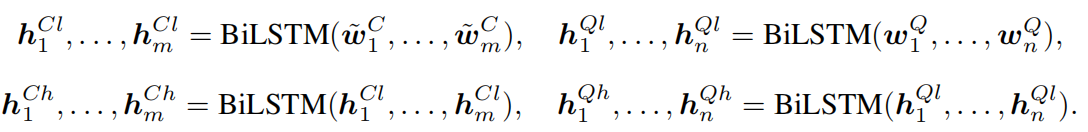
\includegraphics[width=0.7\textwidth]{5-2.png}
		\end{figure}
		\begin{figure}[H]
			\centering
			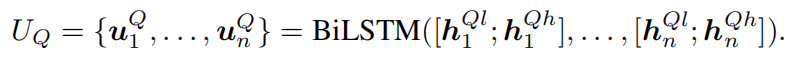
\includegraphics[width=0.5\textwidth]{5-3.png}
		\end{figure}
		
		\subitem[2] Higher-level\\
		\begin{figure}[H]
			\centering
			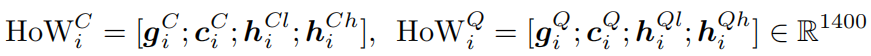
\includegraphics[width=0.5\textwidth]{5-4.png}
		\end{figure}
		\begin{figure}[H]
			\centering
			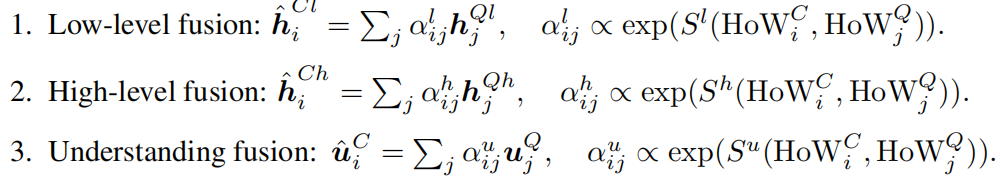
\includegraphics[width=0.6\textwidth]{5-5.png}
		\end{figure}
		\begin{figure}[H]
			\centering
			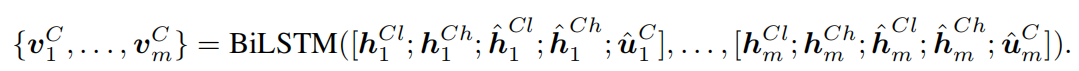
\includegraphics[width=0.6\textwidth]{5-6.png}
		\end{figure}
		\item Fully-Aware Self-Boosted Fusion.\\
		\begin{figure}[H]
			\centering
			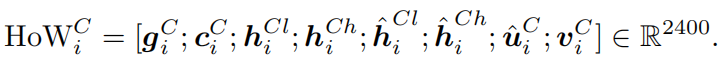
\includegraphics[width=0.5\textwidth]{5-7.png}
		\end{figure}
		\begin{figure}[H]
			\centering
			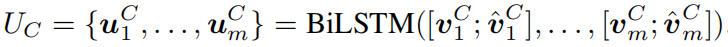
\includegraphics[width=0.5\textwidth]{5-8.png}
		\end{figure}
		\begin{figure}[H]
			\centering
			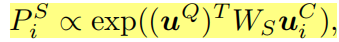
\includegraphics[width=0.3\textwidth]{5-9.png}
		\end{figure}
		\begin{figure}[H]
			\centering
			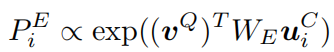
\includegraphics[width=0.3\textwidth]{5-10.png}
		\end{figure}
\end{enumerate}

\newpage
\section{Making Neural QA as Simple as Possible but not Simpler}
典型的神经结构由embedding、encoding、interaction和answer层组成。在本工作中,我们使用上下文/类型匹配启发式作为准则,为抽取QA任务导出简单的神经基线体系结构,提出了基于BoW和BiRNN的baseline,叫做FastQA。\\
【注】启发式算法可以这样定义:一个基于直观或经验构造的算法,在可接受的花费(指计算时间和空间)下给出待解决组合优化问题每一个实例的一个可行解,该可行解与最优解的偏离程度一般不能被预计。
\begin{figure}[H]
	\centering
	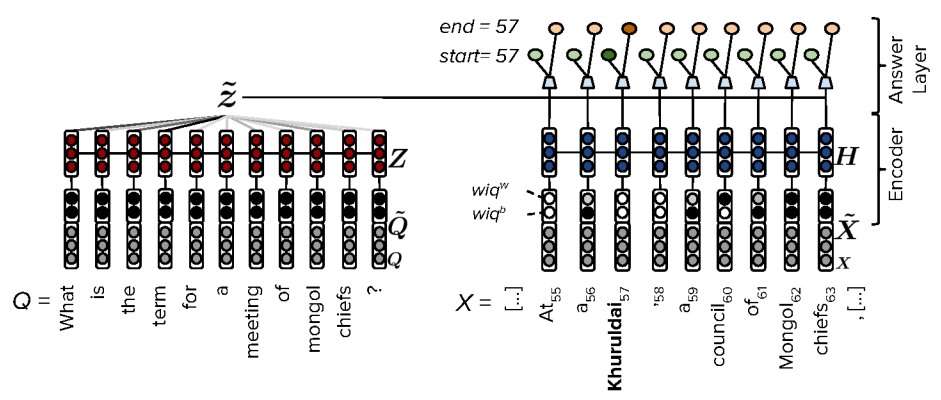
\includegraphics[width=\textwidth]{6-1.png}
\end{figure}
【注】wiq 是指word-in-question feeatures

\newpage
\section{Efficient and Robust Question Answering from Minimal Context over Documents}
研究回答问题所需的最少的context,发现大多数数据集中的问题能够用少量的句子做出回答。因此,提出了一个句子选择器来选出送入QA模型的最小的句子集合。
我们的句子选择器利用了三种简单的技术-权重传递、数据修改和分数归一化,这些技术在句子选择的任务上是非常有效的。\\
\begin{figure}[H]
	\centering
	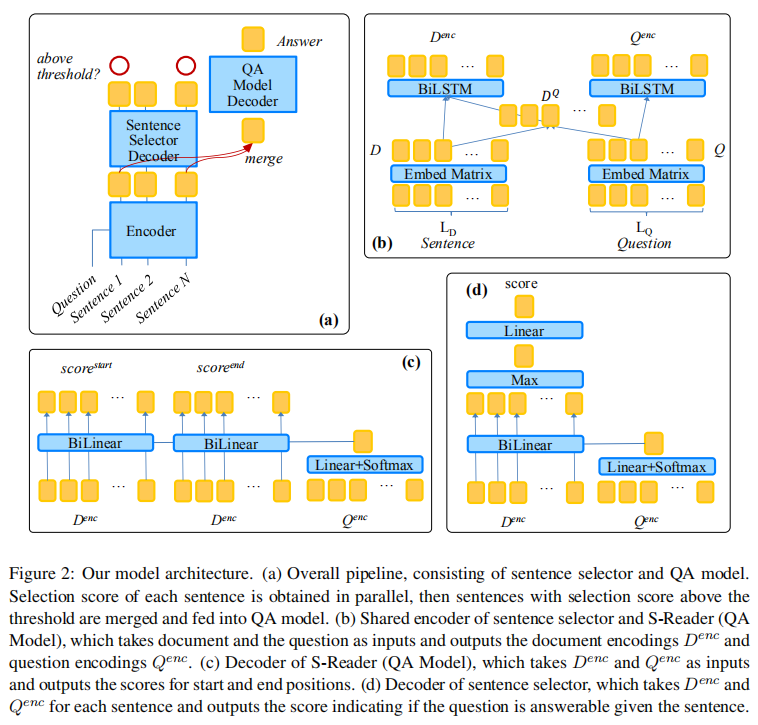
\includegraphics[width=\textwidth]{7-1.png}
	\caption{整体结构图}
\end{figure}
句子选择器并行计算每个句子的选择分数。我们向QA模型提供了一组选择分数较高的简化句子来回答问题,分数代表是否能根据这句话来回答问题。
模型分为encoder模块和decoder模块。
\begin{enumerate}
	\item[(a)] encoder:计算句子和问题的编码。
		\subitem[1] 分别计算sentence embedding $D \in \mathbb{R}^{h_{d} \times L_{d}}$,
		question embedding $Q \in \mathbb{R}^{h_{d} \times L_{q}}$,
		以及question-aware sentence embedding $D^q \in \mathbb{R}^{h_{d} \times L_{d}}$。其中question-aware sentence embedding通过以下方式计算:
		$$
\begin{aligned} \alpha_{i} &=\operatorname{softmax}\left(D_{i}^{T} W_{1} Q\right) \in \mathbb{R}^{L_{q}} \\ D_{i}^{q} &=\sum_{j=1}^{L_{q}}\left(\alpha_{i, j} Q_{j}\right) \in \mathbb{R}^{h_{d}} \end{aligned}
$$		
		\subitem[2] $$
	\begin{aligned} D^{e n c} &=\operatorname{BiLSTM}\left(\left[D_{i} ; D_{i}^{q}\right]\right) \in \mathbb{R}^{h \times L_{d}} \\ Q^{e n c} &=\operatorname{BiLSTM}\left(Q_{j}\right) \in \mathbb{R}^{h \times L_{q}} \end{aligned}
	$$
	\item[(b)] dercoder是一个特定于任务的模块,它通过计算句子编码和问题编码之间的双线性相似性来计算句子的得分,如下所示:
		\subitem[1] 
		$$
\begin{aligned} \beta &=\operatorname{softmax}\left(w^{T} Q^{e n c}\right) \in \mathbb{R}^{L_{q}} \\ q^{\tilde{e} n c} &=\sum_{j=1}^{L_{q}}\left(\beta_{j} Q_{j}^{e n c}\right) \in \mathbb{R}^{h} \end{aligned}
$$
$$
\begin{aligned} \tilde{h}_{i} &=\left(D_{i}^{e n c} W_{2} q^{\tilde{e} n c}\right) \in \mathbb{R}^{h} \\ \tilde{h} &=\max \left(\tilde{h_{1}}, \tilde{h_{2}}, \cdots, h_{L_{d}}\right) \\ \text {score} &=W_{3}^{T} \tilde{h} \in \mathbb{R}^{2} \end{aligned}
$$
\end{enumerate}

\newpage
\section{Simple and Effective Multi-Paragraph Reading Comprehension}
\begin{figure}[H]
	\centering
	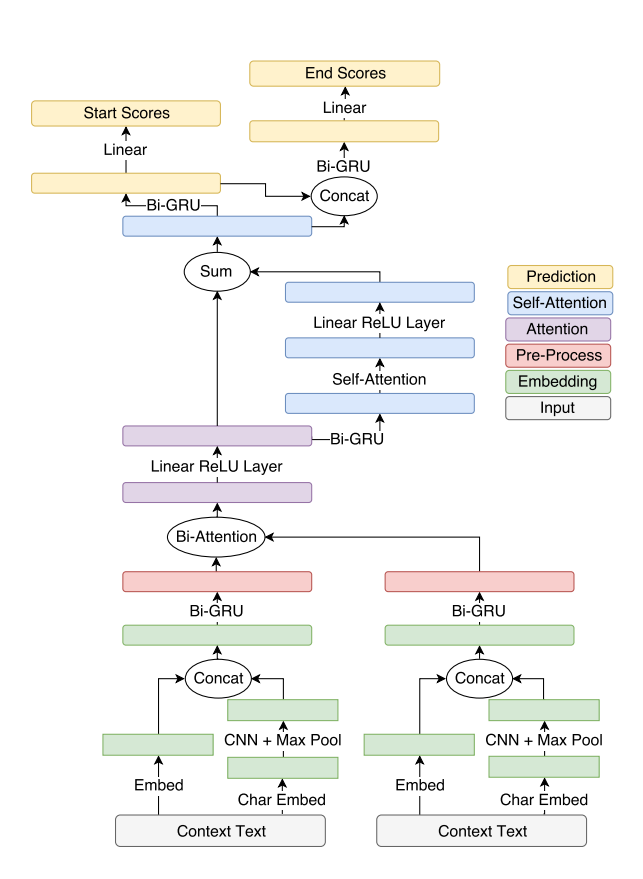
\includegraphics[width=\textwidth]{8-1.png}
\end{figure}
我们介绍了一种将段落级问答模型应用于整个文档作为输入的情况的方法。
我们表明,使用一种改进的训练方案可以显着地提高模型的性能,该方案使模型忽略包含非答案的段落。
我们的方法包括从每个文档中抽取多个段落,并使用一个要求模型生成全局正确输出的目标函数。
\begin{enumerate}
	\item[(a)] Pipelined Method-选择一个段落并将其传递给段落级的问答模型。
	\item[(b)] Condfidence Method-我们使用非归一化和非指数(即在应用Softmax运算符之前)对每个跨度的评分作为模型的度量,将该模型适用于多段设置。 
\end{enumerate}
\newpage
\section{NEURAL SPEED READING VIA SKIM-RNN}
提出了一种新的递归神经网络(RNN),它动态地决定只对相对不重要的输入令牌更新隐藏状态的一小部分。
\begin{figure}[H]
	\centering
	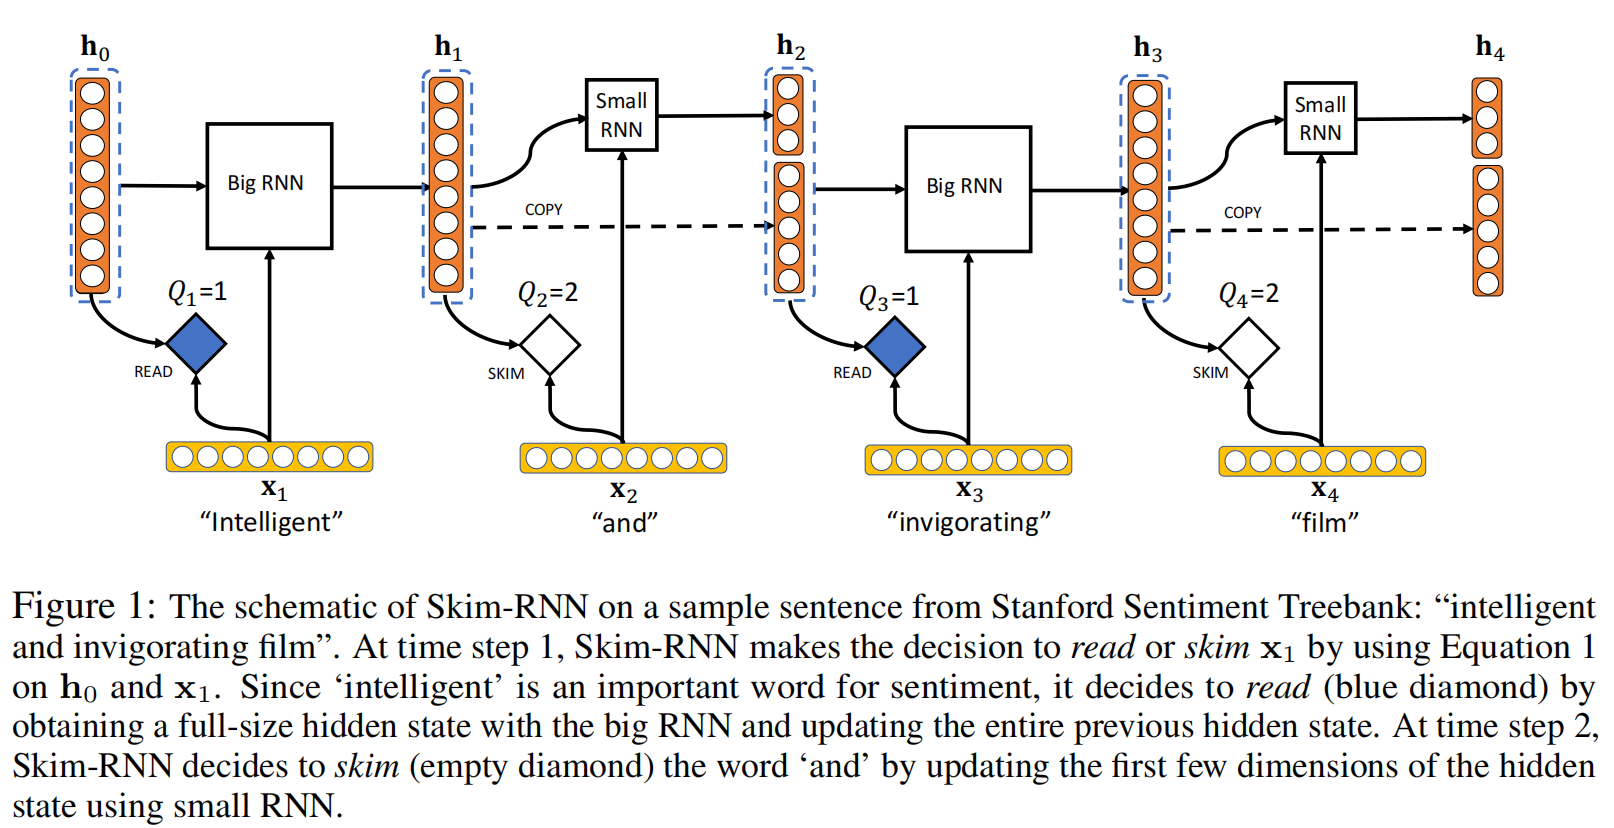
\includegraphics[width=\textwidth]{9-1.png}
\end{figure}
$$
\mathbf{p}_{t}=\operatorname{softmax}\left(\alpha\left(\mathbf{x}_{t}, \mathbf{h}_{t-1}\right)\right)=\operatorname{softmax}\left(\mathbf{W}\left[\mathbf{x}_{t} ; \mathbf{h}_{t-1}\right]+\mathbf{b}\right) \in \mathbb{R}^{k}
$$
$$
Q_{t} \sim \text { Multinomial }\left(\mathbf{p}_{t}\right)
$$
$$
\mathbf{h}_{t}=\left\{\begin{array}{ll}{f\left(\mathbf{x}_{t}, \mathbf{h}_{t-1}\right),} & {\text { if } Q_{t}=1} \\ {\left[f^{\prime}\left(\mathbf{x}_{t}, \mathbf{h}_{t-1}\right) ; \mathbf{h}_{t-1}\left(d^{\prime}+1 : d\right)\right],} & {\text { if } Q_{t}=2}\end{array}\right.
$$
$$
\mathbb{E}_{Q_{t} \sim \operatorname{Multinomial}\left(\mathbf{p}_{t}\right)}[L(\theta)]=\sum_{Q} L(\theta ; Q) P(Q)=\sum_{Q} L(\theta ; Q) \prod_{j} \mathbf{p}_{j}^{Q_{j}}
$$
$$
\mathbf{r}_{t}^{i}=\frac{\exp \left(\left(\log \left(\mathbf{p}_{t}^{i}\right)+g_{t}^{i}\right) / \tau\right)}{\sum_{j} \exp \left(\left(\log \left(\mathbf{p}_{t}^{j}\right)+g_{t}^{j}\right) / \tau\right)}
$$
$$
\mathbf{h}_{t}=\sum_{i} \mathbf{r}_{t}^{i} \tilde{\mathbf{h}}_{t}^{i}
$$
$$
\begin{aligned} \tilde{\mathbf{h}}_{t}^{1} &=f\left(\mathbf{x}_{t}, \mathbf{h}_{t-1}\right) \\ \tilde{\mathbf{h}}_{t}^{2} &=\left[f^{\prime}\left(\mathbf{x}_{t}, \mathbf{h}_{t-1}\right) ; \mathbf{h}_{t-1}\left(d^{\prime}+1 : d\right)\right] \end{aligned}
$$
\newpage
\section{Hierarchical Attention Flow for Multiple-Choice Reading Comprehension}
提出了一个hierarchical attention flow结构,利用候选option的信息来进一步挖掘passage的隐藏信息。
\begin{figure}[H]
	\centering
	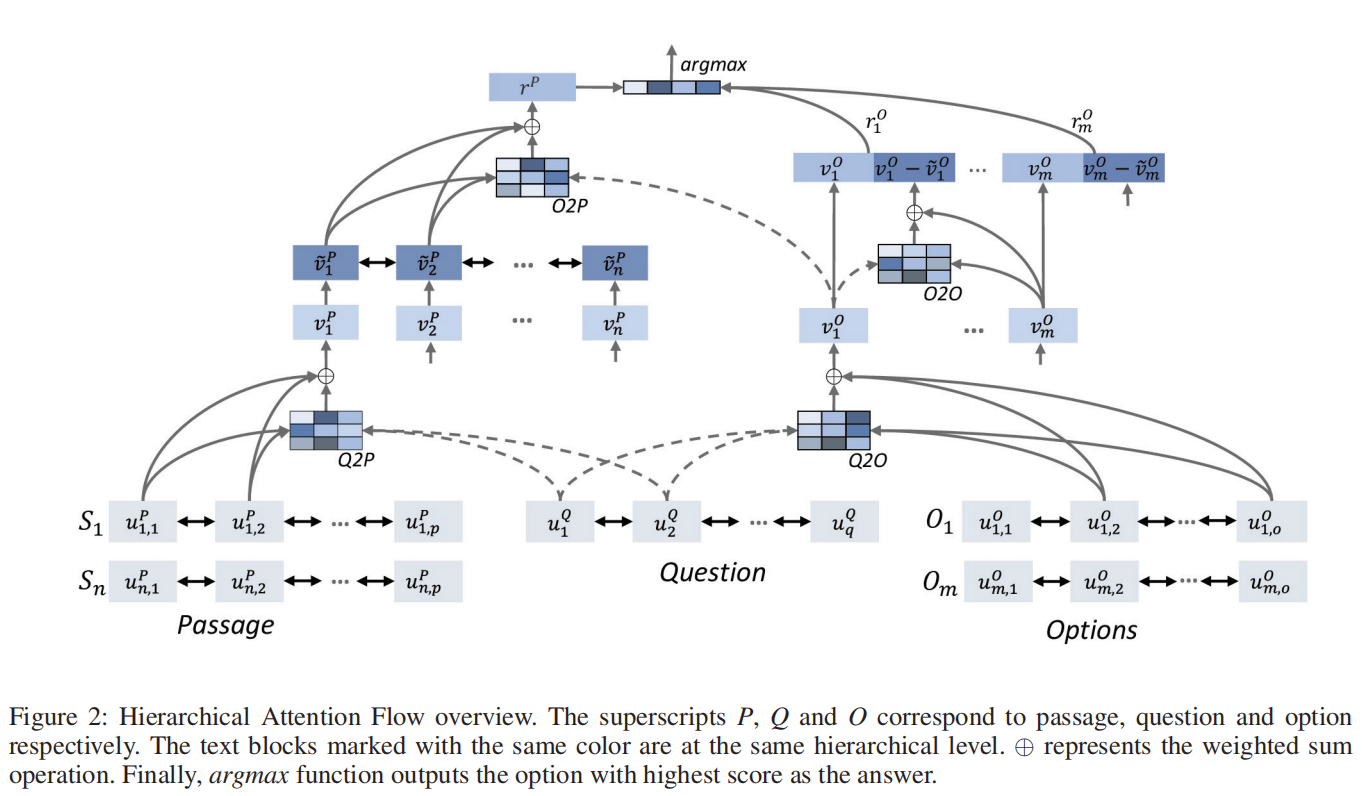
\includegraphics[width=\textwidth]{10-1.png}
\end{figure}
\begin{enumerate}
	\item[1] Word Context Encoder
	\begin{equation}
	\begin{aligned} u_{t}^{Q} &=\operatorname{BiGRU}_{Q}\left(u_{t-1}^{Q}, e_{t}^{Q}\right) \\ u_{i, t}^{P} &=\operatorname{BiGRU}_{P}\left(u_{i, t-1}^{P}, e_{i, t}^{P}\right) \\ u_{i, t}^{O} &=\operatorname{BiGRU}_{O}\left(u_{i, t-1}^{O}, e_{i, t}^{O}\right) \end{aligned}
	\end{equation}
	\item[2] Attention Mechanism
	\begin{equation}
	\begin{array}{c}{A_{i, j}=X_{i} W_{x y} Y_{j}} \\ 
	{s_{i, j}=\frac{\exp \left(A_{i, j}\right)}{\sum_{j}^{n} \exp \left(A_{i, j}\right)}}\\
	a_{j}=\frac{1}{m} \sum_{i=1}^{m} s_{i, j}
	\end{array}
	\end{equation}
	\item[3] Question-to-Passage (Q2P) Word-level Attention
	\begin{equation}
	\begin{array}{c}{a=a t t\left(u^{Q}, u_{i}^{P} | W_{q p}\right)} \\ {v_{i}^{P}=\sum_{t} a_{t} u_{i, t}^{P}}\end{array}
	\end{equation}
	\item[4] Question-to-Option (Q2O) Word-level Attention
	\begin{equation}
	\begin{array}{c}{a=\operatorname{att}\left(u^{Q}, u_{i}^{O} | W_{q o}\right)} \\ {v_{i}^{O}=\sum_{t} a_{t} u_{i, t}^{O}}\end{array}
	\end{equation}
	\item[5] Sentence Context Encoder
	\begin{equation}
		\tilde{v}_{i}^{P}=\operatorname{BiGRU}_{S}\left(\tilde{v}_{i-1}^{P}, v_{i}^{P}\right)
		\end{equation}
	\item[6] Option-to-Passage (O2P) Sentence-level Attention
	\begin{equation}
	\begin{array}{c}{a=a t t\left(v^{O}, \tilde{v}^{P} | W_{o p}\right)} \\ {r^{P}=\sum a_{i} \tilde{v}_{i}^{P}}\end{array}
	\end{equation}
	\item[7] Option Correlations
	\begin{equation}
	\begin{array}{c}{A_{i, j}=v_{i}^{O} W_{o o} v_{j}^{O}} \\ {s_{i, j}=\frac{1(i \neq j) \exp \left(A_{i, j}\right)}{\sum_{j} 1(i \neq j) \exp \left(A_{i, j}\right)}} \\ {\tilde{v}_{i}^{O}=\sum_{j} s_{i, j} v_{j}^{O}} \\ {r_{i}^{O}=\left[v_{i}^{O} ; v_{i}^{O}-\tilde{v}_{i}^{O}\right]}\end{array}
	\end{equation}
	\item[8] answer prediction
	\begin{equation}
	\begin{array}{c}{s_{i}=r^{P} W_{p} r_{i}^{O}} \\ {p_{i}=\frac{\exp \left(s_{i}\right)}{\sum_{j} \exp \left(s_{j}\right)}} \\ {\text {ans}=\operatorname{argmax}_{i}\left(p_{i}\right)}\end{array}
	\end{equation}
\end{enumerate}


\newpage
\section{Towards Reading Comprehension for Long Document}
利用hierarchical—LSTM来学习到paragraph-level的文本表示,从而能够从document中提取答案span,利用匹配机制
找出最有可能含有答案的paragraph。核心就是将每一个paragraph生成一个向量,从而形成paragraph级的文本表示,然后再进行选择。
\begin{figure}[H]
	\centering
	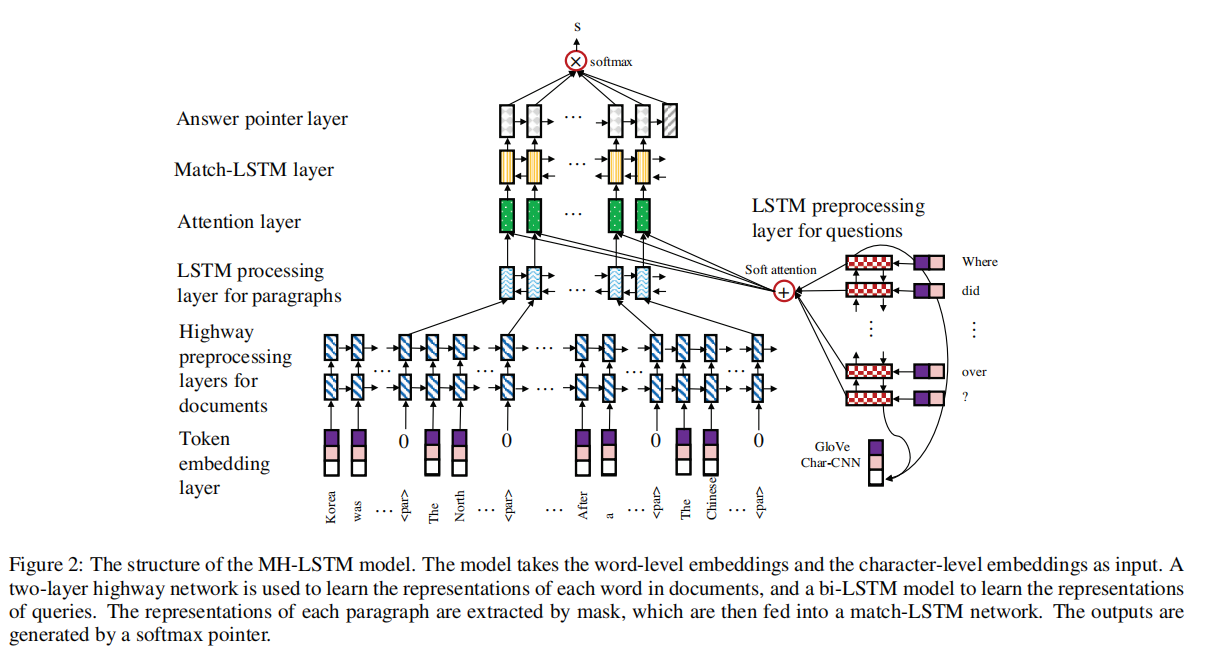
\includegraphics[width=\textwidth]{11-1.png}
\end{figure}
\begin{enumerate}
	\item Token Embedding Layer
	\item Preprocessing Layer for Query
	\begin{equation}
		\mathbf{H}^{Q}, \mathbf{q}_{r e p}=\stackrel{\longleftrightarrow}{\operatorname{LSTM}}(Q)
	\end{equation}
	\item Preprocessing Layer for Context\\
	我们将$q_{rep}$连接到文档中每个单词的嵌入构成$p_t$。
	\begin{equation}
	\begin{array}{c}{\mathbf{s}_{l, t}^{P}=\mathbf{h}_{l, t}^{P} \cdot \mathbf{t}_{l, t}^{P}+\mathbf{s}_{l-1, t}^{P} \cdot \mathbf{c}_{l, t}^{P}} \\ {\mathbf{h}_{l, t}^{P}=\tanh \left(\mathbf{W}_{H}^{P} \mathbf{p}_{t} \mathbb{I}_{\{l=1\}}+\mathbf{R}_{H_{l}}^{P} \mathbf{s}_{l-1, t}^{P}+\mathbf{b}_{H_{l}}^{P}\right)} \\ {\mathbf{t}_{l, t}^{P}=\sigma\left(\mathbf{W}_{T}^{P} \mathbf{p}_{t} \mathbb{I}_{\{l=1\}}+\mathbf{R}_{T_{l}}^{P} \mathbf{s}_{l-1, t}^{P}+\mathbf{b}_{T_{l}}^{P}\right)} \\ {\mathbf{c}_{l, t}^{P}=\sigma\left(\mathbf{W}_{C}^{P} \mathbf{p}_{t} \mathbb{I}_{\{l=1\}}+\mathbf{R}_{C_{l}}^{P} \mathbf{s}_{l-1, t}^{P}+\mathbf{b}_{C_{l}}^{P}\right)}\\\mathbf{H}^{P}=\left[\mathbf{s}_{2,1}^{P}, \ldots, \mathbf{s}_{2,|P|}^{P}\right] \in \mathbb{R}^{h^{P} \times|P|}\end{array}
	\end{equation}
	\item Hierarchical Mask Layer
	\begin{equation}
		\mathbf{H}^{M}=\stackrel{\longleftrightarrow}{\operatorname{LSTM}}\left(\operatorname{mask}\left(\mathbf{H}^{P}\right)\right)=\left[\mathbf{y}_{1}^{M}, \ldots, \mathbf{y}_{|M|}^{M}\right]
		\end{equation}
	\item Attention Layer
	\begin{equation}
	\begin{aligned} \overrightarrow{\mathbf{G}}_{t, i}=& \tanh \left(\overrightarrow{\mathbf{W}^{A Q}} \mathbf{y}_{i}^{Q}+\overrightarrow{\mathbf{W}^{A M}} \mathbf{y}_{t}^{M}+\overrightarrow{\mathbf{b}^{\dot{A}}}\right) \\ \vec{\alpha}_{t} &=\operatorname{softmax}\left(\overrightarrow{\mathbf{w}}^{\top} \overrightarrow{\mathbf{G}}_{t, *}\right) \end{aligned}
	\end{equation}
	\item Match-LSTM Layer
	\begin{equation}
	\begin{array}{c}{\overrightarrow{\mathrm{y}}_{t}=\overrightarrow{\mathrm{LSTM}}\left(\overrightarrow{\mathrm{z}}_{t}, \overrightarrow{\mathrm{y}}_{t-1}\right)} \\ {\overrightarrow{\mathrm{z}}_{t}=\left[\begin{array}{c}{\mathbf{y}_{t}^{M}} \\ {\mathbf{H}^{Q} \vec{\alpha}_{t}^{\top}}\end{array}\right]}\\\overrightarrow{\mathbf{G}}_{t, i}=\tanh \left(\overrightarrow{\mathbf{W}^{A Q}} \mathbf{y}_{i}^{Q}+\overrightarrow{\mathbf{W}^{A M}} \mathbf{y}_{t}^{M}+\overrightarrow{\mathbf{W}^{A O}} \mathbf{y}_{t}+\overrightarrow{\mathbf{b}^{A}}\right)\end{array}
	\end{equation}
	\item Output Pointer Layer
	\begin{equation}
	\begin{array}{c}{\left[\mathbf{y}_{1}^{e}, \ldots, \mathbf{y}_{|M|}^{e}\right], \mathbf{e}_{r e p}=\text { ENCODER }\left(\mathbf{H}^{O}\right)} \\ {\mathbf{y}^{d}=\operatorname{DECODER}\left(\mathbf{e}_{r e p}\right)}\end{array}
	\end{equation}
	\item Training
	\begin{equation}
		L(\theta)=-\frac{1}{N} \sum_{n=1}^{N} \log p\left(\widetilde{a_{n}} | \widetilde{P_{n}}, \widetilde{Q_{n}}\right)=-\frac{1}{N} \sum_{n=1}^{N} \log \mathbf{s}_{\widehat{a_{n}} | \widetilde{P_{n}}, \widetilde{Q_{n}}}
		\end{equation}
\end{enumerate}



\newpage
\section{Joint Training of Candidate Extraction and Answer Selection for Reading Comprehension}
大多数方法以独立的方式对答案进行建模,而忽略了它与其他candidate之间的关系。本文提出了一个两阶段的阅读理解框架:extract-then-select。
我们首先从段落中提取答案候选人,然后结合所有candidata的信息选择最终答案,此外,我们将候选提取作为一个潜在变量,将两阶段过程与强化学习结合起来进行训练。

\begin{figure}[H]
	\centering
	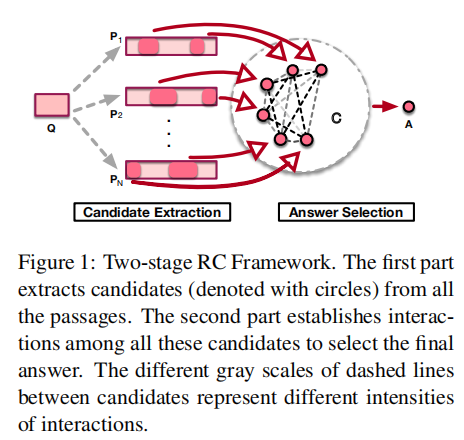
\includegraphics[width=0.5\textwidth]{12-1.png}
\end{figure}
\begin{figure}[htbp]
	\centering

	\subfigure[]{
	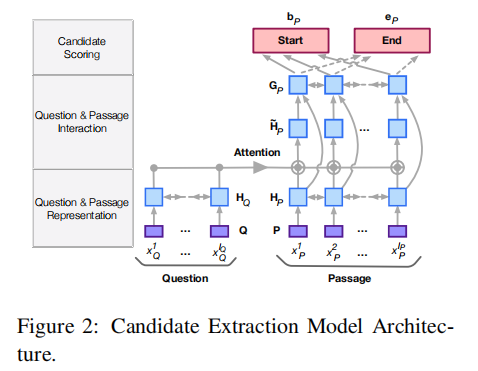
\includegraphics[width=0.45\textwidth]{12-2.png}
	}
	\quad
	\subfigure[]{
	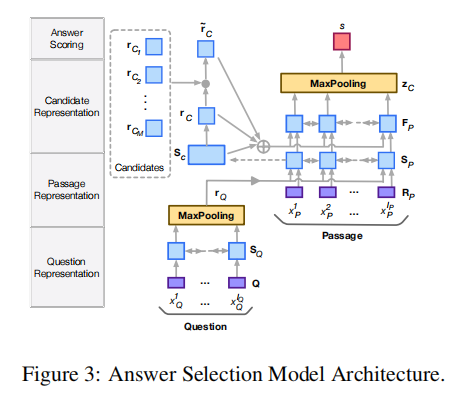
\includegraphics[width=0.45\textwidth]{12-3.png}
	}
	\quad
\end{figure}

\newpage
\section{Multi-Passage Machine Reading Comprehension with Cross-Passage Answer Verification}
multi-passage相比single Passage更加具有挑战性。我们提出了一种端到端的神经模型,使来自不同段落的答案候选人能够根据内容表示相互验证。
我们联合训练了三个模块,它们可以根据三个因素来预测最终答案:答案边界、答案内容和交叉答案验证。
\begin{figure}[H]
	\centering
	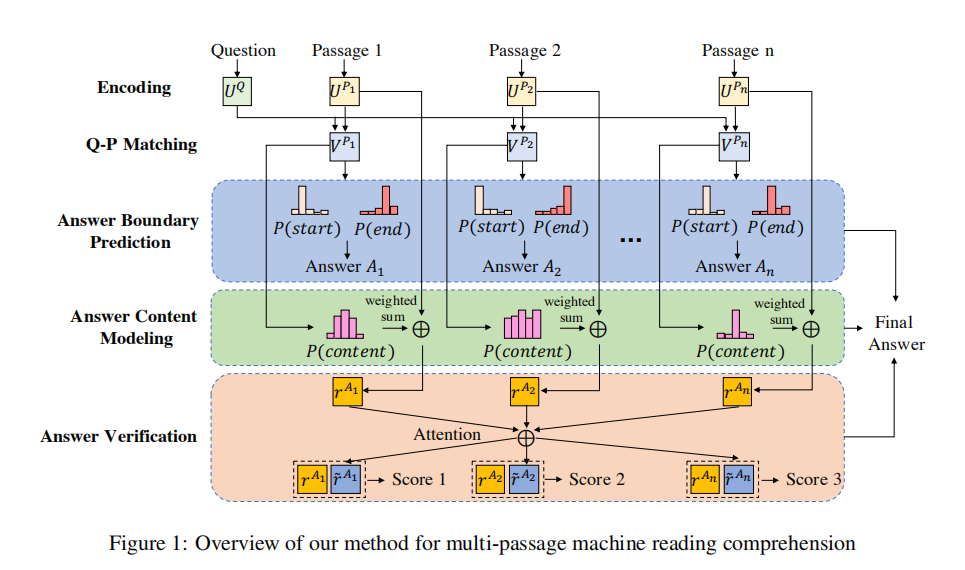
\includegraphics[width=\textwidth]{13-1.png}
\end{figure}
\begin{enumerate}
	\item Answer Boundary Prediction
	\begin{equation}
	\begin{aligned} g_{k}^{t} &=\mathbf{w}_{1}^{a} \mathrm{T} \tanh \left(\mathbf{W}_{2}^{a}\left[\mathbf{v}_{k}^{P}, \mathbf{h}_{t-1}^{a}\right]\right) \\ \alpha_{k}^{t} &=\exp \left(g_{k}^{t}\right) / \sum_{j=1}^{|\mathbf{P}|} \exp \left(g_{j}^{t}\right) \\ \mathbf{c}_{t} &=\sum_{k=1}^{|\mathbf{P}|} \alpha_{k}^{t} \mathbf{v}_{k}^{P} \\ \mathbf{h}_{t}^{a} &=\operatorname{LSTM}\left(\mathbf{h}_{t-1}^{a}, \mathbf{c}_{t}\right) \end{aligned}
	\end{equation}
	\item Answer Content Modeling
	\begin{equation}
		p_{k}^{c}=\operatorname{sigmoid}\left(\mathbf{w}_{1}^{c \top} \operatorname{ReLU}\left(\mathbf{W}_{2}^{c} \mathbf{v}_{k}^{P_{i}}\right)\right)
		\end{equation}
		\begin{equation}
			\mathbf{r}^{A_{i}}=\frac{1}{\left|\mathbf{P}_{i}\right|} \sum_{k=1}^{\left|\mathbf{P}_{i}\right|} p_{k}^{c}\left[\mathbf{e}_{k}^{P_{i}}, \mathbf{c}_{k}^{P_{i}}\right]
			\end{equation}
	\item Cross-Passage Answer Verification
	\begin{equation}
	s_{i, j}=\left\{\begin{array}{ll}{0,} & {\text { if } i=j} \\ {\mathbf{r}^{A_{i} \top} \cdot \mathbf{r}^{A_{j}},} & {\text { otherwise }}\end{array}\right.
	\end{equation}
	\begin{equation}
	\begin{aligned} \alpha_{i, j} &=\exp \left(s_{i, j}\right) / \sum_{k=1}^{n} \exp \left(s_{i, k}\right) \\ \tilde{\mathbf{r}}^{A_{i}} &=\sum_{j=1}^{n} \alpha_{i, j} \mathbf{r}^{A_{j}} \end{aligned}
	\end{equation}

	\begin{equation}
		g_{i}^{v}=\mathbf{w}^{v \top}\left[\mathbf{r}^{A_{i}}, \tilde{\mathbf{r}}^{A_{i}}, \mathbf{r}^{A_{i}} \odot \tilde{\mathbf{r}}^{A_{i}}\right]
		\end{equation}
		\begin{equation}
			p_{i}^{v}=\exp \left(g_{i}^{v}\right) / \sum_{j=1}^{n} \exp \left(g_{j}^{v}\right)
			\end{equation}
\end{enumerate}


\newpage
\section{Reinforced Mnemonic Reader for Machine Reading Comprehension}
首先提出了一种reattention机制,能够访问临时存储的multi-round对齐的过去的attentions,来细化当前的注意力。
另外提出了一种新的优化方式,叫做dynamic-critical reinforcement learning,它总是鼓励预测一个更可接受的答案,以解决传统的强化学习算法中存在的收敛抑制问题。
\begin{figure}[H]
	\centering
	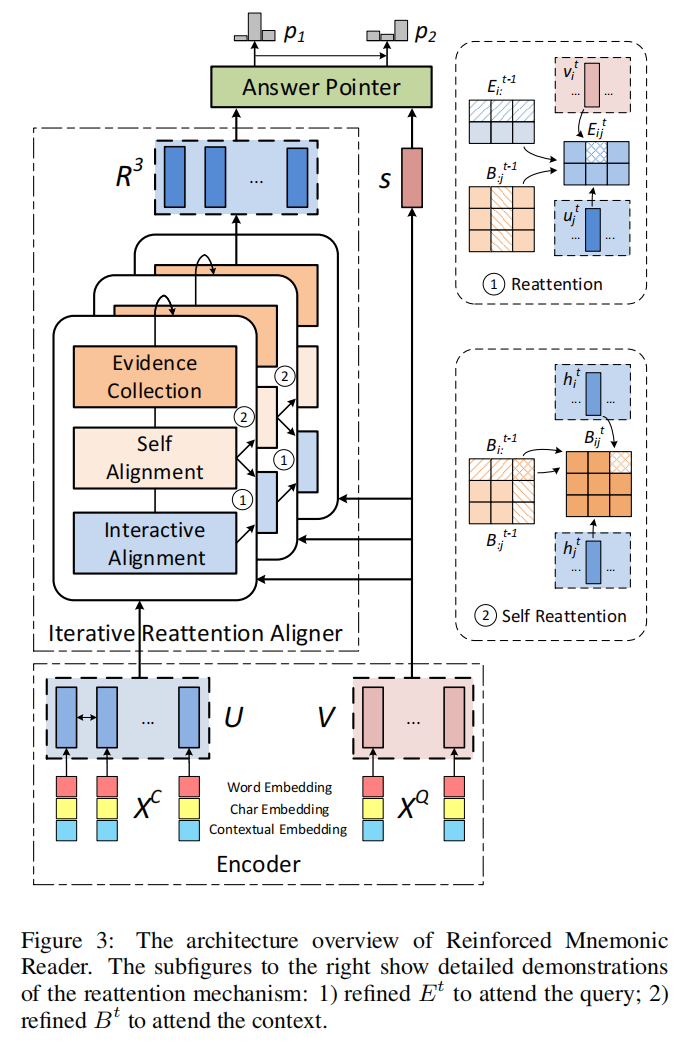
\includegraphics[width=0.8\textwidth]{14-1.png}
\end{figure}
\begin{enumerate}
	\item Reattention Mechanism\\
	\begin{equation}
	\begin{array}{l}{\tilde{E}_{i j}^{t}=\operatorname{softmax}\left(E_{i :}^{t-1}\right) \cdot \operatorname{softmax}\left(B_{ : j}^{t-1}\right)} \\ {E_{i j}^{t}=f\left(v_{i}^{t}, u_{j}^{t}\right)+\gamma \tilde{E}_{i j}^{t}}\end{array}
	\end{equation}
	\begin{equation}
	\begin{array}{l}{\tilde{B}_{i j}^{t}=\operatorname{softmax}\left(B_{i :}^{t-1}\right) \cdot \operatorname{softmax}\left(B_{ : j}^{t-1}\right)} \\ {B_{i j}^{t}=\mathbb{1}_{(i \neq j)}\left(f\left(h_{i}^{t}, h_{j}^{t}\right)+\gamma \tilde{B}_{i j}^{t}\right)}\end{array}
	\end{equation}
	\item Dynamic-critical Reinforcement Learning
	\item End-to-end Architecture\\
	\begin{equation}
	\begin{array}{c}{\tilde{x}=\operatorname{relu}\left(W_{r}[x ; y ; x \circ y ; x-y]\right)} \\ {g=\sigma\left(W_{g}[x ; y ; x \circ y ; x-y]\right)} \\ {o=g \circ \tilde{x}+(1-g) \circ x}\end{array}
	\end{equation}
	\begin{equation}
	\begin{array}{c}{R^{1}, Z^{1}, E^{1}, B^{1}=\operatorname{align}^{1}(U, V)} \\ {R^{2}, Z^{2}, E^{2}, B^{2}=\operatorname{align}^{2}\left(R^{1}, V, E^{1}, B^{1}\right)} \\ {R^{3}, Z^{3}, E^{3}, B^{3}=\operatorname{align}^{3}\left(R^{2}, V, E^{2}, B^{2}, Z^{1}, Z^{2}\right)}\end{array}
	\end{equation}
	\begin{figure}[H]
		\centering
		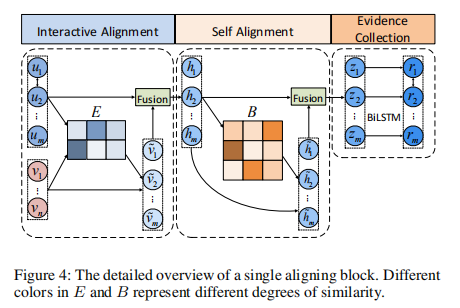
\includegraphics[width=0.5\textwidth]{14-2.png}
	\end{figure}
\end{enumerate}
\end{document}